\clearpage
\section{Who changes groups, and why?}\label{sec:cases}
A change in membership is easiest to understand at household level. Cluster numbers themselves cannot be compared across independently fitted models. We first match Product labels to RFM labels by maximum household overlap, then inspect households whose matched assignments differ. From each direction of change, we select the household nearest its transition group's centroid in the transformed Product feature space, breaking distance ties by household identifier. The selection uses calibration data only. The comparison concerns the full enrichment from RFM to Product, including basket behavior; it cannot attribute every change to department preferences alone.

After alignment, 287 of 2,498 households (11.5\%) change groups: 163 move from RFM's lower-activity group to Product's higher-activity group, and 124 move in the reverse direction. These are cross-model reassignments of the same calibration households, not changes over time.

\textbf{Household 2389: broader shopping despite less recent activity.} This household last purchased 33 days before the reference day, made 43 baskets and recorded 1,102.61 in sales. Its 342 products across 13 departments accompany a move from the lower RFM group to the higher Product group. Meat accounts for 12.9\% of spending and Produce 7.8\%. The richer representation incorporates breadth and basket behavior that RFM does not explicitly encode.

\textbf{Household 1970: recent visits with smaller baskets.} With recency of seven days and 44 baskets, this household moves from the higher RFM group to the lower Product group. Recorded sales total 615.01; mean basket sales are 13.98, compared with 25.64 for household 2389. Grocery and Drug GM account for 66.5\% and 17.9\% of spending, with 214 products across eight departments. Similar visit counts therefore need not imply similar basket scale or mix.

Both the basket variables and the department block change between RFM and Product, so these examples do not isolate the effect of one variable.

\begin{figure}[htbp]\centering
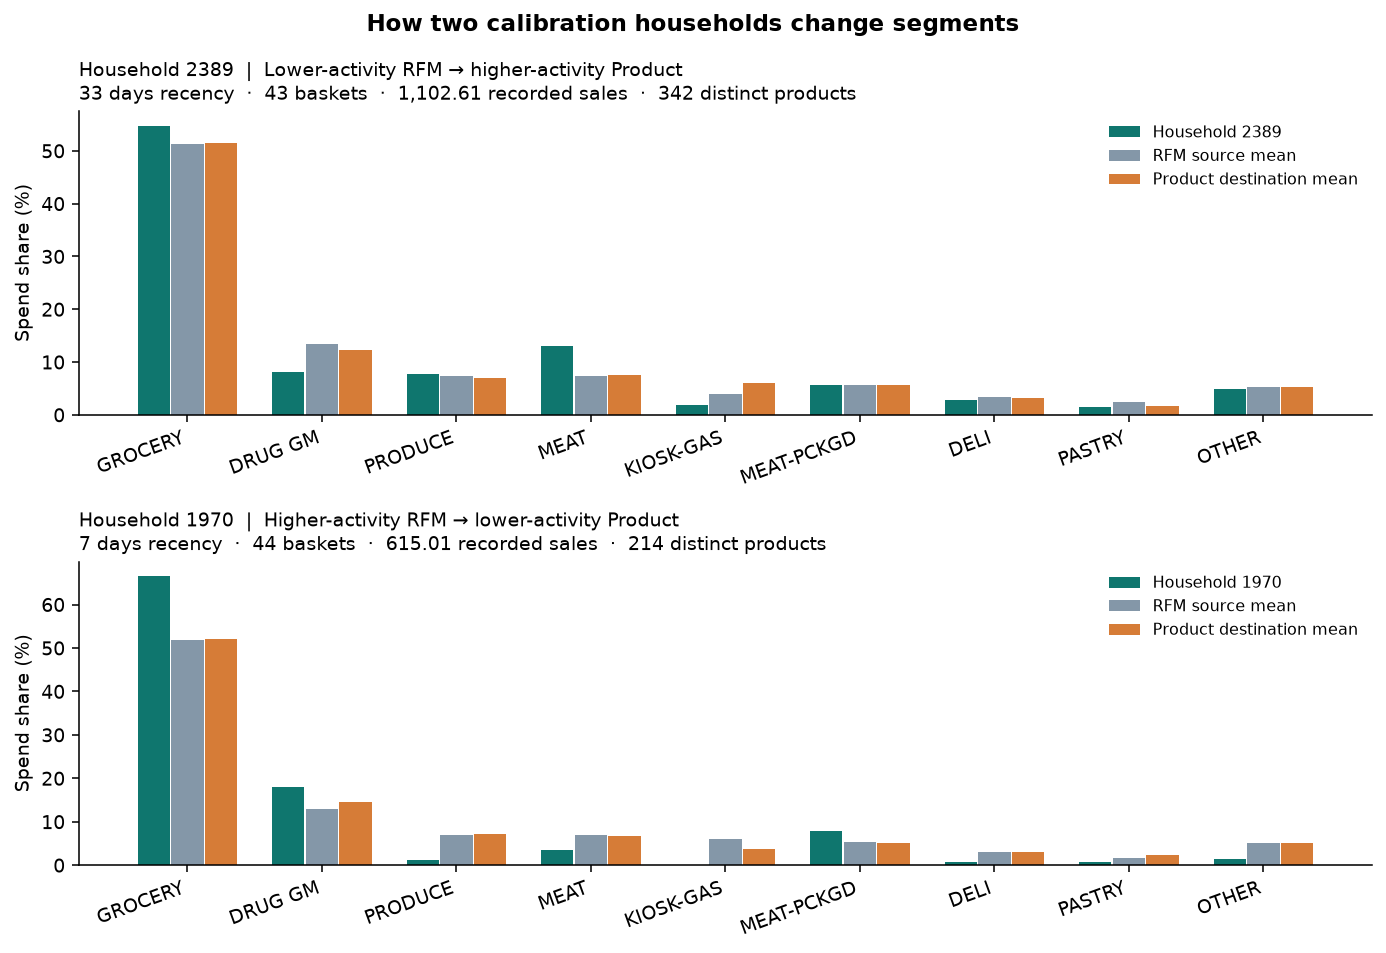
\includegraphics[width=\textwidth]{../figures/10_household_cases.png}
\caption{Actual calibration households selected by a reproducible rule from the changed-membership groups. Sales and basket counts describe the calibration period only. These cases illustrate how different definitions of similarity change a household's assignment.}\label{fig:cases}
\end{figure}

\section{Do department differences persist later?}\label{sec:futurecategories}
The original later-spending criterion is naturally related to RFM's monetary feature. We therefore add a category-specific descriptive check: do the frozen groups distinguish later department spending shares? This extension was designed after the original holdout results had been inspected. It is exploratory and leaves the original feature fitting, cluster-count selection and frozen memberships unchanged.

The category vocabulary remains the eight largest calibration departments plus Other. Later purchases in any department outside that vocabulary enter Other. We calculate each household's department shares separately and give each household equal weight. Shares are undefined for the 59 calibration households with no positive later purchase: they remain in the full-cohort spending and activity results, but the category-composition comparison uses the same 2,439 active households for every representation. This separates absence of purchases from preference for a department.

\begin{figure}[htbp]\centering
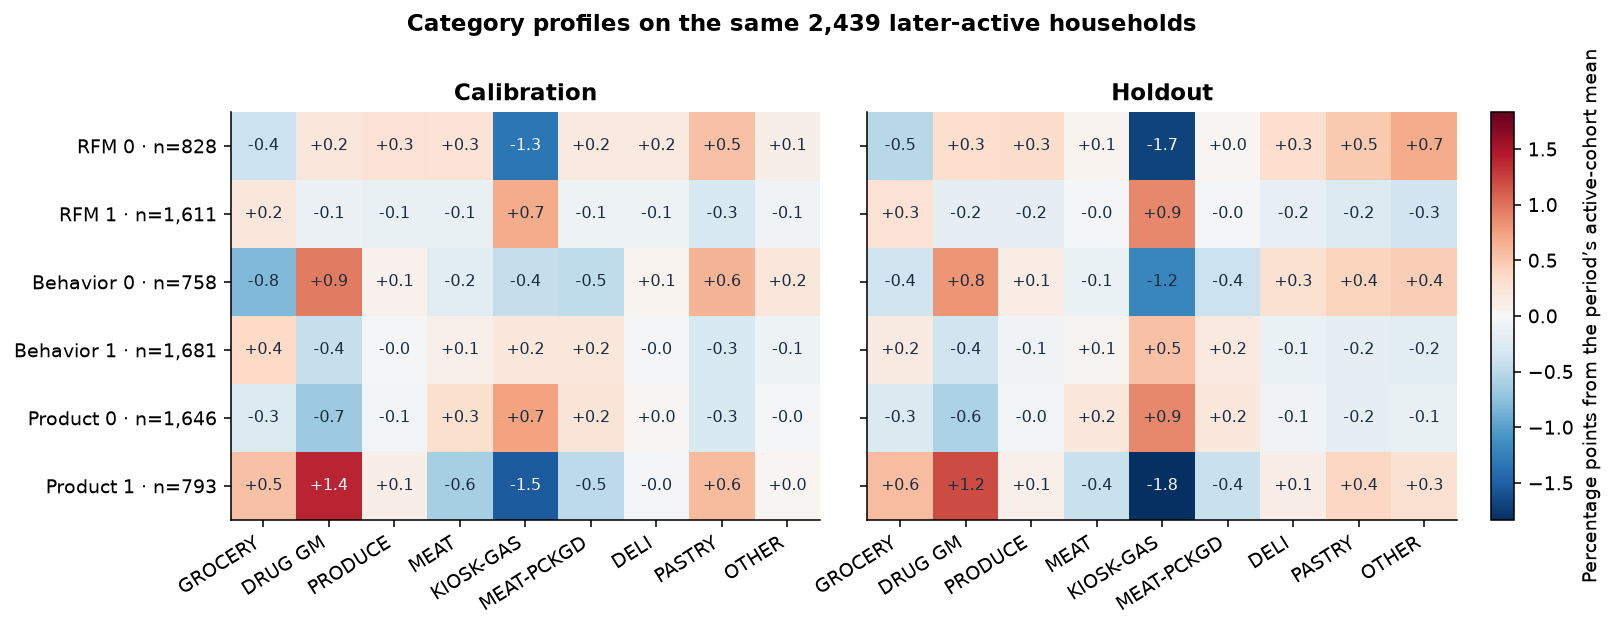
\includegraphics[width=\textwidth]{../figures/12_future_categories.png}
\caption{Department-share deviations for frozen groups. Calibration and later profiles use the same later-active household cohort, with each period centered on that cohort's mean household share. A repeated direction of deviation suggests persistence.}\label{fig:futurecategories}
\end{figure}

For household share vector $\mathbf{s}_i$ and frozen group $g$, the category separation measure is
\[
\eta^2_{\mathrm{category}}=
\frac{\sum_g n_g\lVert\overline{\mathbf{s}}_g-\overline{\mathbf{s}}\rVert^2}
{\sum_i\lVert\mathbf{s}_i-\overline{\mathbf{s}}\rVert^2}.
\]
It is the fraction of total squared variation in nine-component household shares that lies between group means. This raw-share Euclidean summary weights departments by their observed variation. We compare Product minus RFM using 1,000 paired household bootstrap replicates (seed 2027), keeping fitted memberships fixed.

\begin{table}[htbp]\centering
\caption{Exploratory category-share separation on the identical 2,439 later-active households. Entries are percentages of total squared share variation explained by frozen group means, not percentages of shoppers or sales.}\label{tab:categoryholdout}
\begin{tabular}{lrr}\toprule
Representation & Calibration & Later period\\\midrule
RFM & 0.250\% & 0.299\%\\
Behavior & 0.221\% & 0.180\%\\
Product & 0.529\% & 0.386\%\\\bottomrule
\end{tabular}
\end{table}

Product has the largest point estimate for later category separation, but it explains only 0.386\% of the total variation in household shares, versus 0.299\% for RFM. The Product-minus-RFM difference is $0.000868$ on the fraction scale (0.087 percentage points), with a conditional 95\% interval of $[-0.001097,0.003148]$. The interval spans zero, so there is no clear improvement.

Some profile directions do persist. Among the later-active cohort, Product's lower-activity group is 1.39 percentage points above the calibration cohort mean for Drug GM and 1.20 points above the later mean. Its Kiosk-Gas deviations are $-1.53$ and $-1.83$ points respectively. Persistence is not universal: its small Deli deviation changes sign.

\textbf{What this adds to the decision.} Even against department preferences rather than later spending, the two-group Product model shows only a small advantage. Retain RFM for broad activity monitoring and use category profiles as supplementary descriptions.
